\documentclass[titlepage]{article}
\usepackage[colorlinks=true]{hyperref}
\usepackage{graphicx}
\usepackage{caption}
\begin{document}
%simple command to add a figure 
%\myfigure{address}{caption}{width}
\newcommand{\myfigure}[3]{
\begin{figure}[h!]
  \centering
  \includegraphics[width=#3\textwidth]{#1}
  \caption{#2}
\end{figure}
}
\title{\huge KUKA Youbot Autonomous Robot: Controls and Planning Technical Plan}
\author{Ze Che\\
 \and
Chenkai Shao\\
\and
Edward Aguilar\\
\and
Ivan Jimenez\\
\and
Abraham Marsen\\
\and
Myron Lee}
\large\date{January 30, 2014\endgraf\bigskip\hrule\bigskip
Georgia Institute of Technology (GT)\\
GT Vertically Integrated Projects (VIP)\\
Georgia Tech Research Institute (GTRI)\\
GTRI Robotics VIP Team
}
\maketitle
\tableofcontents
\newpage
\section{Introduction}
In the field of agriculture, there is a constant issue of labor cost vs consumer prices. Because of the naturally erratic nature of plant-life, harvesting presents a particularly complex problem to both hardware and software and has thus been left to seasonal workers, which in both recent and coming years has driven the price of produce up as the wage of these workers has risen. With this in mind, it is imperative that a system to replace these costs step in to fill the gap in order to keep consumer prices down. Already, there are products out there that are in the early stages of this task, with examples such as the Intelligent Robotic Vineyard Pruner from Vision Robotics Corp. and Wall-Ye V.I.N. by Christopher Millot serving the needs of wine-makers and the Robotic Strawberry Harvester by Robotic Harvesting, LLC serving to collect strawberries.
\begin{figure}[h!]
\centering
\begin{minipage}{.5\textwidth}
  \centering
  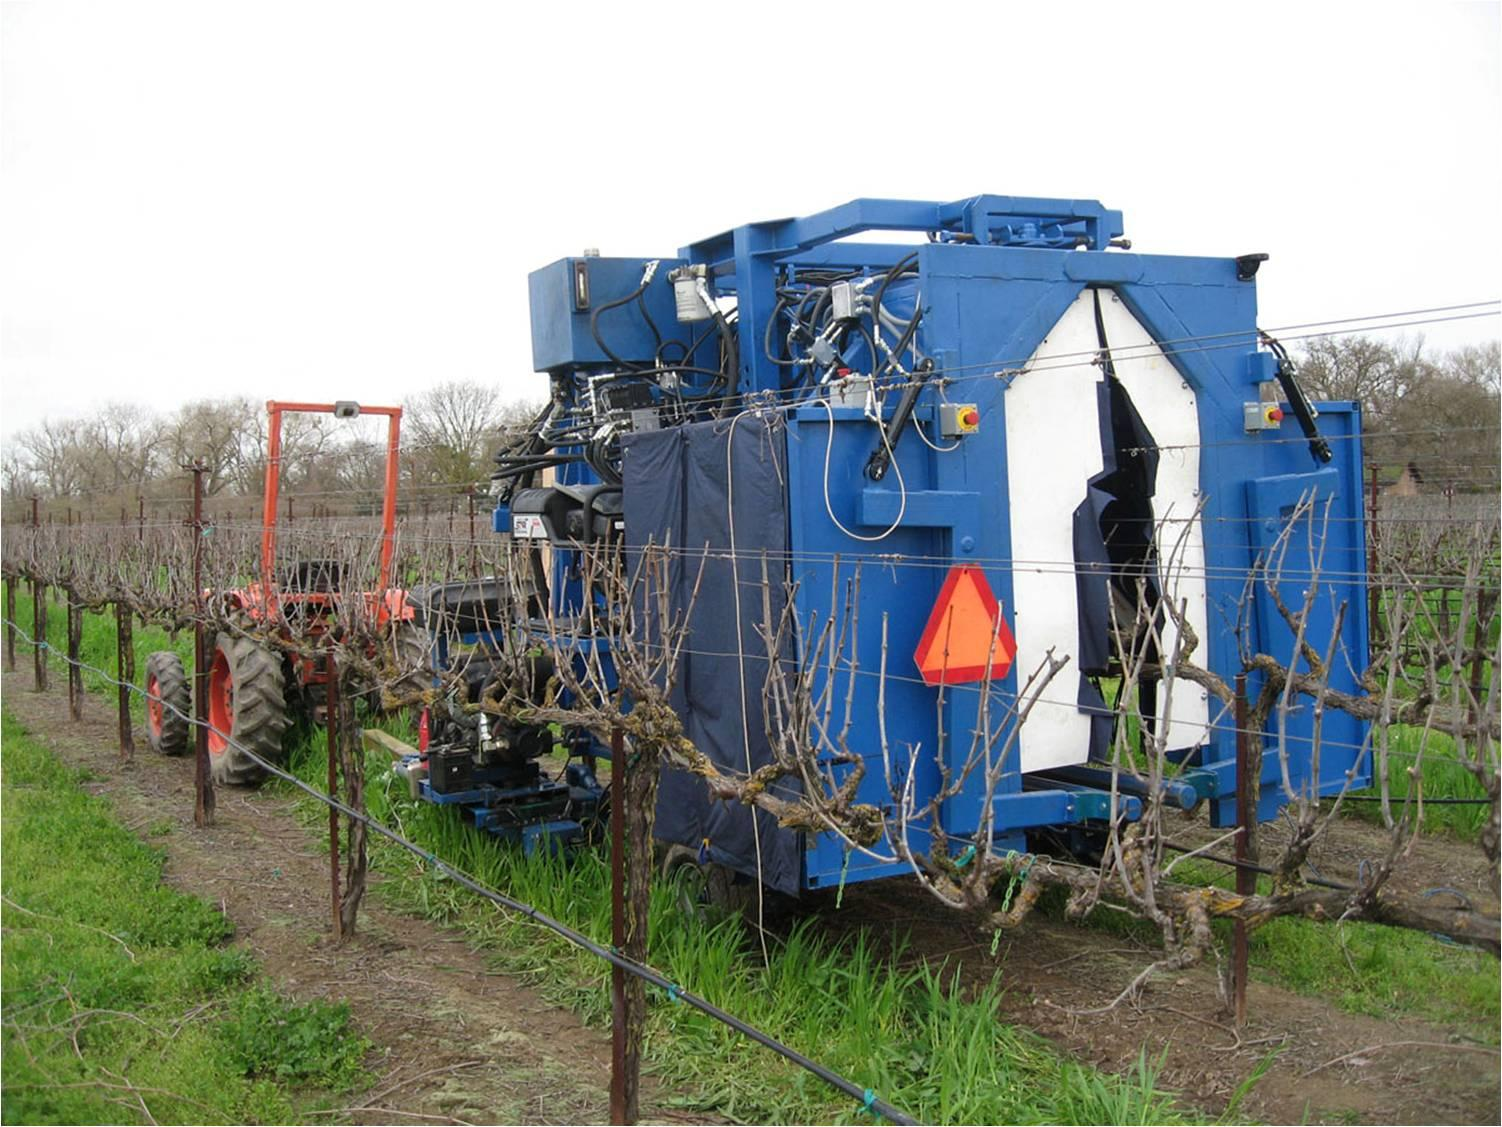
\includegraphics[width=.8\linewidth]{Images/blueTrain.jpg}
  \captionof{figure}{blue train}
\end{minipage}%
\begin{minipage}{.5\textwidth}
  \centering
  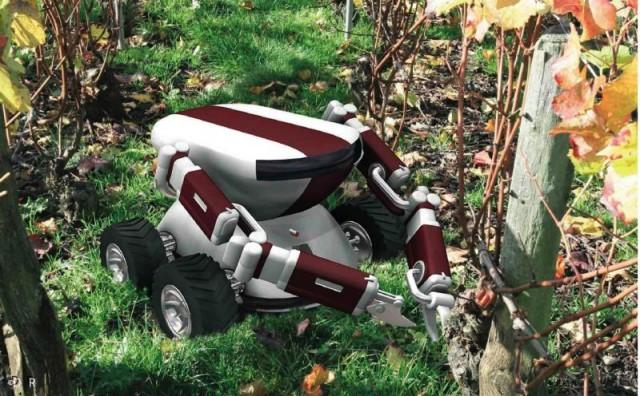
\includegraphics[width=.8\linewidth]{Images/brownrobot.jpg}
  \captionof{figure}{brown robot}
\end{minipage}
\end{figure}
However, as previously stated, the simple task of picking produce is very complicated. In general, an automated system must be able to first distinguish that the produce exists amongst other real-world objects, then go through a series of motions and information transactions in order to retrieve the produce safely, then navigate its sensors to the next possible location of produce to start the process over again.

\myfigure{Images/greenTracktor.jpg}{Robotic Strawberry Harvester by Robotic Harvesting, LLC}{.5}

With this in mind, the goal of this research is to produce a system by which an autonomous robot can, after detection of its target, maneuver a robotic arm through obstacles to capture and retrieve the detected produce. When used in concert with the work from our Perception and Mapping team developments through the robot produced by our Modification team, our target will be a green bell pepper, but it is planned that the robot will be able to function with other produce targets and will be able to be tailored to other robots of similar construction. The boon this will offer to the agricultural industry is obvious, as it greatly reduces the cost to only the initial price of the robot, power, and the manpower necessary to provide maintenance for the machine, which may be left to warranty or the owner.
\section{Goals}
When completed, the program will be able to process location data from a world map for navigation, know when a target has been perceived, guide the picking arm to its target in real time, and plot and execute a route to the location of a potential target. These tasks will be broken up as follows:
\begin{enumerate}
\item Robot path finding
\begin{enumerate}
\item Process World Mapping
\item Steer and Drive
\end{enumerate}
\item Target detection
\begin{enumerate}
\item Process Perception
\end{enumerate}
\item Target retrieval
\begin{enumerate}
\item Instruct Robot Arm
\end{enumerate}
\end{enumerate}
In the long term, it is planned that the program will be able to operate for a variety of similar produce types with no changes other than the target to be detected, but will be easily alterable if alternative hardware is required for the produce retrieval. The end result will be the navigation to a bell pepper plant, the detection of a ripe fruit, and the harvesting of that fruit without damage.

\section{Background}
\section{Details}
\subsection{Controller Design}
Each joint of the Youbot has its motor controller. Specifically, each motor controller contains an ARM Cortex-M3 microcontroller, Hall Sensors, EtherCAT interfaces, and PID-Controllers. The PID-Controllers are further separated into position, velocity, and current PID-Controllers. Also, each joint has an I2t monitor that determines the square of the sum of the motor current over a period of time for safety measures. The control parameters have already been optimized and allows for relatively faster response time compared to the more common PI-Controllers. For simplicity, the group will begin by exploring the position controller and its related Youbot APIs.
\myfigure{Images/PositionController.png}{Position Controller in which the n stands for motor positions, e for errors, and other variables are optimized parameters.}{1}
\subsection{Youbot API}
The Youbot API consists of C++ open source libraries not only provides access to full firmware functionality, but also support joint level control. From commanding and sensing joint values including position, velocity, and current to manually tuning each joint parameter, the Youbot API provides a simple and direct method for implementing and testing mentioned planning algorithms. While the Youbot API supports base movement in the Cartesian space, the manipulator movement within the Cartesian space is not supported. Furthermore, the API does not provide any forward or inverse kinematics functionalities. From previous semester’s research, a possible inverse kinematic solution is the OpenRave IKFast library.   As part of the ROS framework, the IKFast conveniently outputs the necessary parameters Youbot joint command-calls require through numerical solving techniques.

Another important aspect of the Youbot API is that it encapsulates EtherCAT communication. Along with the EthercatMaster, the API provides a method of communication between the user application and the Youbot. Running an API with communication thread usually has a default cycle time of 1ms while running the API without a constant communication thread requires manual calls to methods such as sendProcessData() and receiveProcessData() scheduled by a real-time operating system (RTOS).
\myfigure{Images/youbotDriverOverview.png}{Diagram describing the communication threads and interactions within Youbot and between Youbot and user applications.}{.5}
\subsection{Search Algorithms}
\subsubsection{Graph Traversal Algorithms}
Finding the best shortest path in a workspace for a robot can be both challenging and frustrating. There are many processes that go into account concerning motion planning for the robot. Encompassing many applications, autonomy is the important key for our project as our goal is to create an autonomous robotic system. Motion planning algorithms are thus crucial in order to produce a continuous motion while avoiding collisions. One of the algorithms we will be considering is A* which is one of the most popular choices for pathfinding due to its flexibility. A* uses a best-first search, which is a search algorithm that navigates a graph of one or more goal points, or nodes. Like other graph-searching algorithms, in which it is capable of searching a huge area, one of the first steps before the beginning of the A* algorithm would be to simplify the search area before finding the path. At the starting point, a search is conducted taking into account the nodes around. Once the surrounding area is taken into account, the starting point is designated as a point of no interest or a closed node since the next step would be to take the first step on the path to the ending goal.
\myfigure{Images/planningProblem.png}{A model of the search area.}{.5}
Which direction to take is the question that is taken into consideration as the algorithm ranks the points surrounding the starting point on a certain basis. This basis is determined by two parameters, with one determining if the vertices are closer or farther than the starting point relative to the ending point and the other incorporating the use of heuristics. By using heuristics, an estimated distance from the remaining path can be calculated, which will help us develop the shortest path possible. Using these two parameters repeatedly will eventually form a path of possible points to take, and when taking into account any obstacles, the path will begin to unveil itself. These ranks the parameters establish can be modeled by a function, f(n) = g(n) + h(n) where g(n) reveals a cost to move from the starting point to a given node and h(n) reveals the heuristic. The steps to the path are used by the approach of maintaining an open nodes and closed nodes list. By keeping track of whether A* has already visited a node, A* will continue searching until the ending point has been reached or if for some reason the open nodes list is empty in which case there is no path.
\myfigure{Images/planningSolution.png}{A\* revealing the path to the goal}{.5}
While A* is widely used, there are other algorithms to take into account as well. D* is another approach in searching and pathfinding. In contrast to A*, D* begins searching by working backwards from the goal point. By producing a path based on given and assumed data, a path can be created while it is progressively updated due to any new information given about its surrounding area. This process is repeated until the destination coordinates are reached or if it’s been determined that there is no possible path. Similar to A*, D* maintains a list of nodes that are marked by a certain condition to be analyzed. RAISE and LOWER are two states specific to D* in which they reveal the cost of a node to be either higher or lower than the previous cost. Before a cost can be increased, the algorithm will check the neighboring nodes and observe if a deduction cost can be taken. If it is not possible, the RAISE state will spread among the nodes that contain backpointers which aid in developing the path. A backpointer denotes the next node directing to the target. The path will eventually be unveiled by following the backpointers. D* proves to be an efficient search algorithm while A* provides the shortest, lowest cost path, therefore it will be interesting to see which algorithm will work the best for our project.
\myfigure{Images/DStarMap.png}{A map revealing a path created by D\*}{.5}
\section{Collaboration}
Since the team’s responsibilities span from planning the robots route to implementing and controlling the robot’s movement, it is easier for other sub-teams to picture this team’s pipeline as a “black box”. Information transfer and implementation within the team will be independent from the processes of the other sub-teams. The idea is to create an application with the necessary APIs to communicate with other teams while dealing with inputs from other teams within our application. Specifics of the interfaces between other sub-teams will have to be discussed during the beginning phases of the project. It is crucial for each sub-team to recognize required inputs and possible output formats. For example, in order to generate the best route using mapping team’s data, the planning team will have to be able to process the output data for the map. Will the agreed format be .vtk generated from navigation meshes (the mapping algorithm from previous semester) or will the mapping team decide to explore other possible mapping algorithms? Questions like these will have to answer through cross-team discussion in order to successfully implement the interface.

Information from the mapping team will be utilized to generate the most efficient route possible. The team expects some sort of map data communicated through agreed APIs and will utilize the data to generate the route through its own thread processes. After receiving the needed poses, the control team will be responsible of moving the robot and this will provide the perception team with the updated coordinates of the robot without any explicit output from the controls team.   

Aside from weekly meetings that will allow each team to update their progresses, urgent questions regarding implementation details can be posted and answered utilizing the team’s forum. With each team member capable of posting questions, answers, and follow-ups, confusion about other team’s work can be minimized. Furthermore, blog posts regarding each individual’s work on his/her research will also allow teammates to understand the technology and research utilized during the progression of the project.
\section{Conclusion}
\begin{thebibliography}{20}
\bibitem{RRT} \href{http://msl.cs.uiuc.edu/rrt/papers.html}{Rapidly-Exploring Random Trees}
\end{thebibliography}

\end{document}
